\section{Etapa de verificación}
La metodología que se utilizó en este proyecto fue la metodología Kanban, gracias a esta se pudo realizar con mayor facilidad esta etapa.

Para llevar a cabo la metodología se utilizó Microsoft Planner, una herramienta que ayuda con la gestión de proyectos. Aquí se creó un tablero que contiene 4 columnas y cada una de las columnas contiene las tarjetas con las actividades (Ver Figura 51).

    \begin{figure}[H]
        \begin{center}
            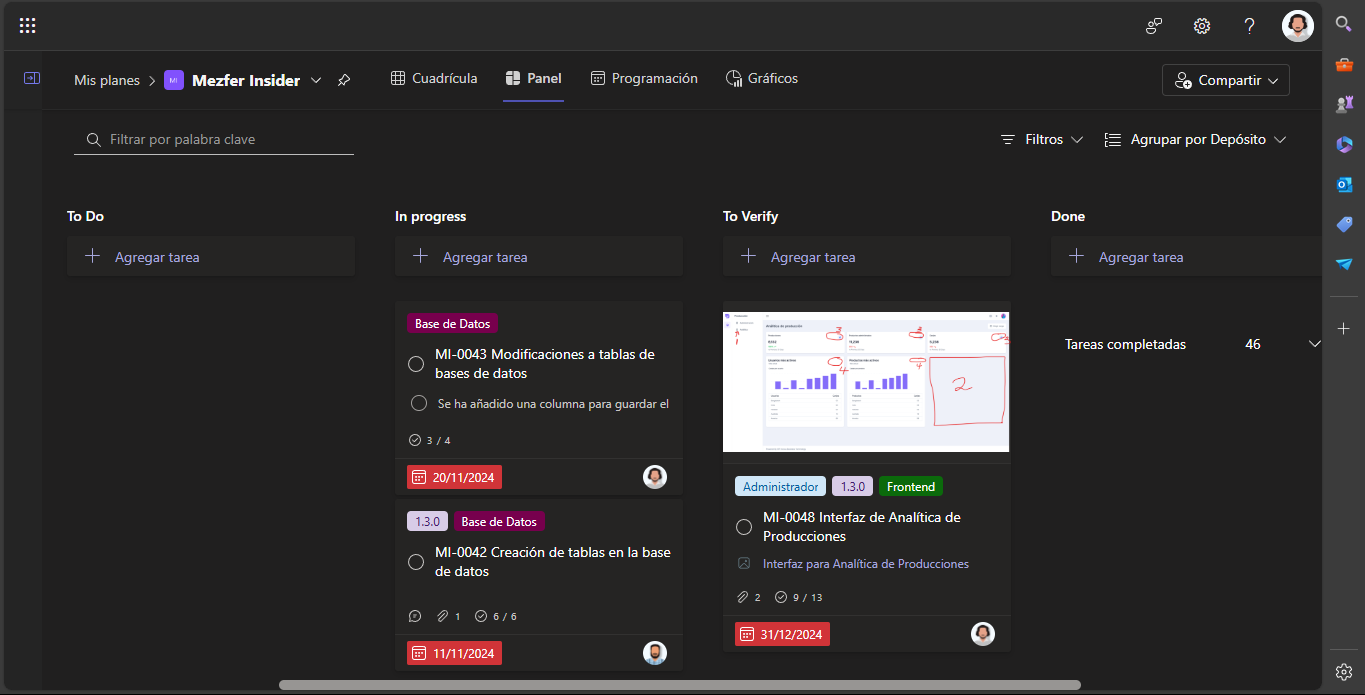
\includegraphics[scale=0.35]{img/resultados/tablero-kanban.png}
            \caption{Ejemplo de tablero kanban.}
            \label{fig:tablero-kanban}
        \end{center}
    \end{figure}

Las columnas que se encuentran en el tablero son:
    \begin{itemize}
        \item To Do: Aquí se colocan las tarjetas con las actividades que se van a realizar en cierto periodo de tiempo.
        \item In Progress: Aquí están las tarjetas con las actividades que se están desarrollando.
        \item To Verify: Las tarjetas que se encuentran en esta columna estan listas para ser comprobadas. Aquí se revisará si se cumplen todos los requerimientos de la actividad.
        \item Done: Aquí se colocan las tarjetas cuyos requerimientos se han cumplido satisfactoriamente y, por lo tanto, se consideran finalizadas.
    \end{itemize}

Las tarjetas contienen información que es útil para realizar la actividad. Entre la información que se puede encontrar en la tarjeta está:
    \begin{itemize}
        \item Nombre de la actividad
        \item Fecha de inicio
        \item Fecha de finalización
        \item Encargado de la actividad
        \item Importancia
        \item Descripción
        \item Lista de verificación
        \item Archivos adjuntos
    \end{itemize}

Cuando las tarjetas se encontraban en la columna ``To Verify'', se convocaba a una reunión para realizar una revisión. Como guía para esta revisión se utilizaban las listas de verificación de las tarjetas, de esta manera se iban marcando como completados los requerimientos hasta que todos se cumplieran; en caso de que algunos no se cumplieran, las tarjetas eran regresadas a la columna ``In Progress'' para completar los requerimientos faltantes.